\documentclass{article}%
\usepackage[T1]{fontenc}%
\usepackage[utf8]{inputenc}%
\usepackage{lmodern}%
\usepackage{textcomp}%
\usepackage{lastpage}%
\usepackage[head=40pt,margin=0.5in,bottom=0.6in]{geometry}%
\usepackage{graphicx}%
%
\title{\textbf{Personal del Metro de Caracas interrumpió protesta~de comité de usuarios}}%
\author{El Nacional Web}%
\date{28/09/2018}%
%
\begin{document}%
\normalsize%
\maketitle%
\textbf{URL: }%
http://www.el{-}nacional.com/noticias/protestas/personal{-}del{-}metro{-}caracas{-}interrumpio{-}protestade{-}comite{-}usuarios\_253560\newline%
%
\textbf{Periodico: }%
EN, %
ID: %
253560, %
Seccion: %
Protestas\newline%
%
\textbf{Palabras Claves: }%
NO\_TIENE\newline%
%
\textbf{Derecho: }%
2.3, %
Otros Derechos: %
, %
Sub Derechos: %
2.3.1\newline%
%
\textbf{EP: }%
SI\newline%
\newline%
%
\textbf{\textit{Carlos Julio Rojas, coordinador del Frente en Defensa del Norte de la capital, ofrecía declaraciones cuando fue abordado por un trabajador del sistema subterráneo}}%
\newline%
\newline%
%
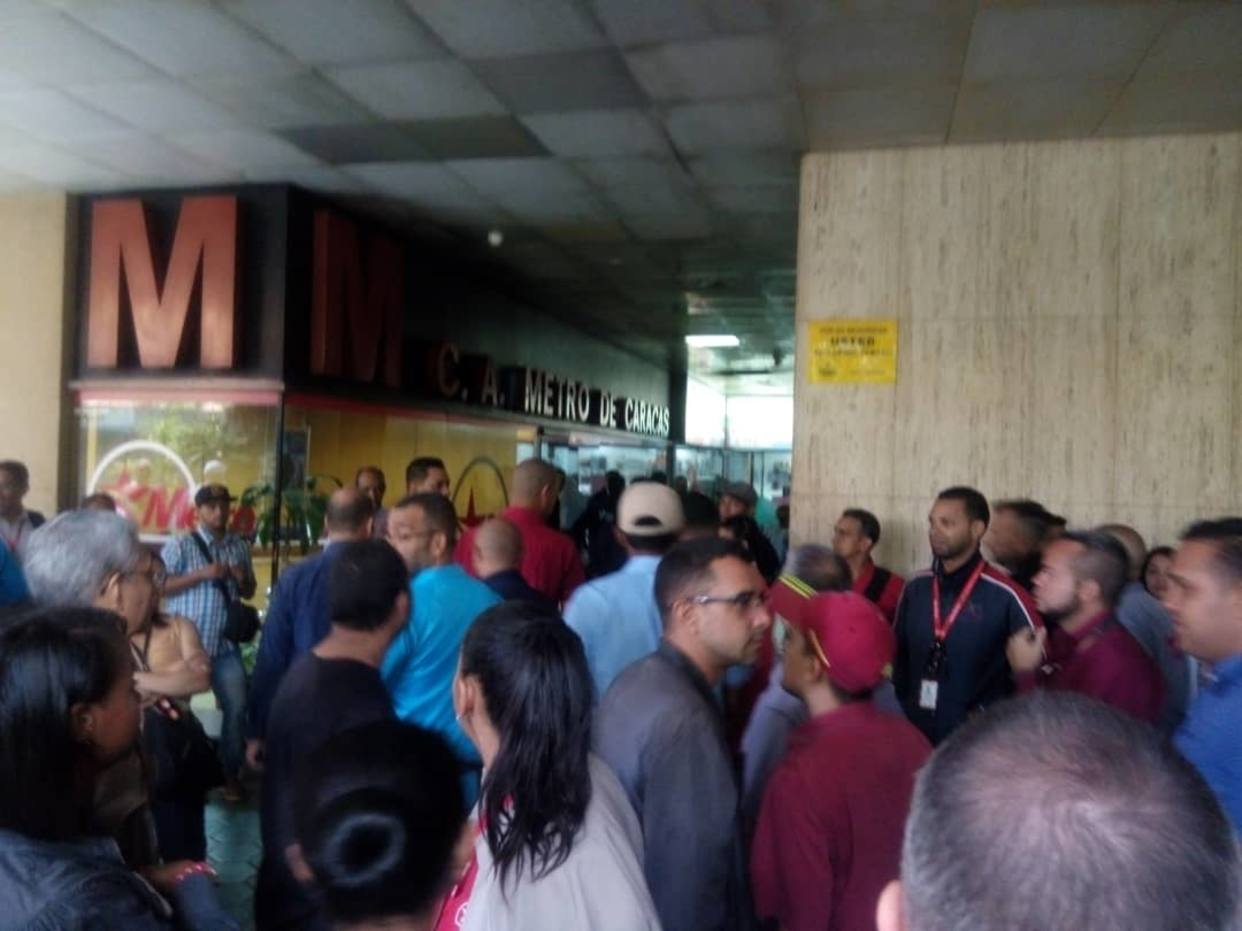
\includegraphics[width=300px]{49.jpg}%
\newline%
%
Personal del Metro de Caracas interrumpió una protesta que realizaban miembros del comité~en defensa del transporte público afuera del despacho del presidente del sistema subterráneo.%
\newline%
%
El Coordinador del Frente en Defensa del Norte de Caracas, Carlos Julio Rojas aseguró que como usuario tiene derecho a expresarse ante la calidad del servicio de transporte.%
\newline%
%
“60\% de los empleados del Metro renunciaron porque ganaban un salario miserable, esto demuestra que hay un cierre técnico del sistema subterráneo”, detalló luego de ser abordado por un trabajador del Metro.%
\newline%
%
Los manifestantes entregararon~un documento en el que~se describen las fallas que presenta el sistema.%
\newline%
%
\end{document}